\subsection{Pi}

Bilens styreenhed er valgt til at være en Raspberry Pi, da denne er et oplagt valg da imlementeringen både skal indeholde videostreaming og socketbaseret netværkskommunikation. Der er altså tale om en højniveau controller. Pi'en er ligeledes forsynet med et kamara\cite{lib:cam} og en Wi-Fi dongle\cite{lib:wifi}. Funktionaliteten udvikles i et program der er bestående er flere klasser, der kan ses på figur \ref{fig:cd_pi}, som herefter vil beskrives meget kort. Foruden det program som er udviklet af projektgruppen selv, anvendes et tredjepartsprogram, kaldet Motion\cite{lib:motion-on-raspberry} til at streame videoen. For flere detaljer end nedenstående henvises til \ref{P-ch:softwaredesign} \nameref{P-ch:softwaredesign} pi side \pageref{P-ch:softwaredesign} og \ref{P-ch:sw_impl} \nameref{P-ch:sw_impl} på side \pageref{P-ch:sw_impl}.

\begin{figure}[h]
\centering
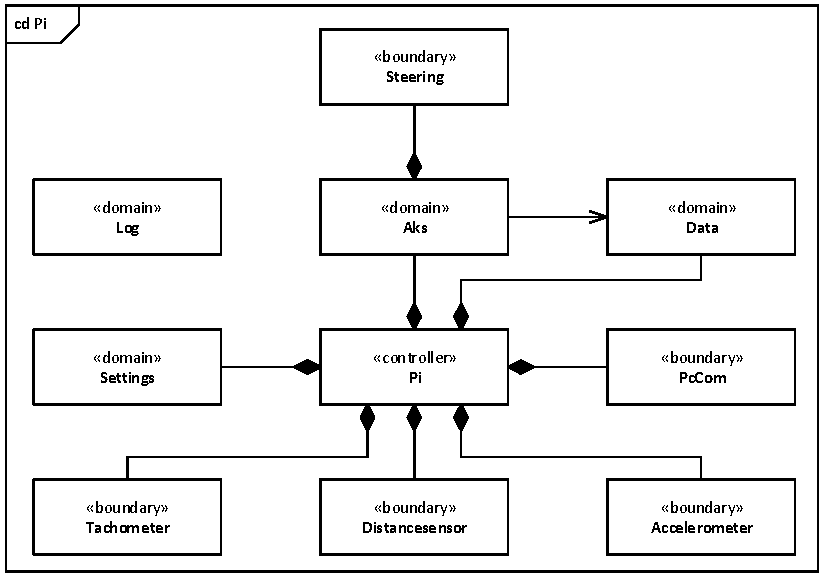
\includegraphics[width=\textwidth* 9/10]{../fig/diagrammer/bil/cd_pi.pdf}
\caption{Klassediagram over Pi}
\label{fig:cd_pi}
\end{figure}

Der gøres opmærksom på at samtlige klaser i klassediagrammet på figur \ref{fig:cd_pi} har en association til Log-klassen. Det er undladt at tegne alle disse pile, da dette vil uoverskueliggøre diagrammet.


\subsection{Pi}

Bilens styreenhed er valgt til at være en Raspberry Pi, da denne er et oplagt valg da imlementeringen både skal indeholde videostreaming og socketbaseret netværkskommunikation. Der er altså tale om en højniveau controller. Pi'en er ligeledes forsynet med et kamara\cite{lib:cam} og en Wi-Fi dongle\cite{lib:wifi}. Funktionaliteten udvikles i et program der er bestående er flere klasser, der kan ses på figur \ref{fig:cd_pi}, som herefter vil beskrives meget kort. Foruden det program som er udviklet af projektgruppen selv, anvendes et tredjepartsprogram, kaldet Motion\cite{lib:motion-on-raspberry} til at streame videoen. For flere detaljer end nedenstående henvises til \ref{P-ch:softwaredesign} \nameref{P-ch:softwaredesign} pi side \pageref{P-ch:softwaredesign} og \ref{P-ch:sw_impl} \nameref{P-ch:sw_impl} på side \pageref{P-ch:sw_impl}.

\begin{figure}[h]
\centering
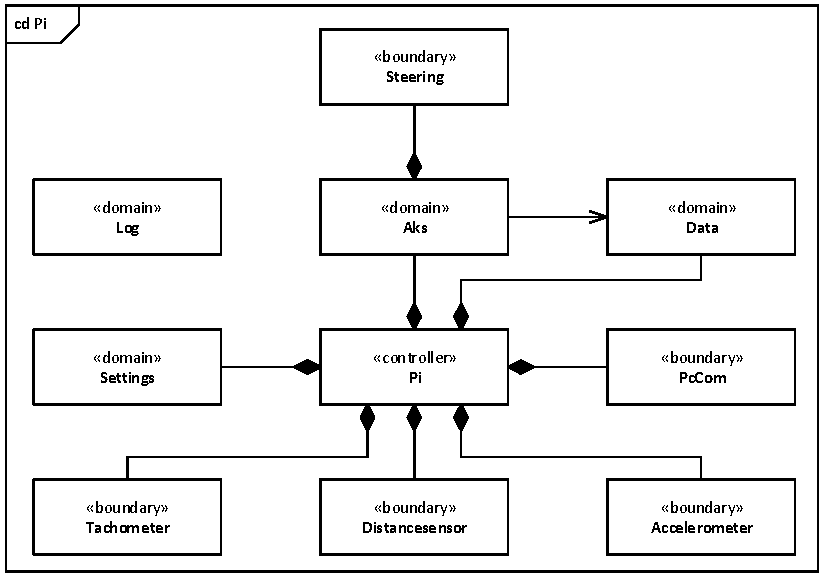
\includegraphics[width=\textwidth* 9/10]{../fig/diagrammer/bil/cd_pi.pdf}
\caption{Klassediagram over Pi}
\label{fig:cd_pi}
\end{figure}

Der gøres opmærksom på at samtlige klaser i klassediagrammet på figur \ref{fig:cd_pi} har en association til Log-klassen. Det er undladt at tegne alle disse pile, da dette vil uoverskueliggøre diagrammet.


\subsection{Pi}

Bilens styreenhed er valgt til at være en Raspberry Pi, da denne er et oplagt valg da imlementeringen både skal indeholde videostreaming og socketbaseret netværkskommunikation. Der er altså tale om en højniveau controller. Pi'en er ligeledes forsynet med et kamara\cite{lib:cam} og en Wi-Fi dongle\cite{lib:wifi}. Funktionaliteten udvikles i et program der er bestående er flere klasser, der kan ses på figur \ref{fig:cd_pi}, som herefter vil beskrives meget kort. Foruden det program som er udviklet af projektgruppen selv, anvendes et tredjepartsprogram, kaldet Motion\cite{lib:motion-on-raspberry} til at streame videoen. For flere detaljer end nedenstående henvises til \ref{P-ch:softwaredesign} \nameref{P-ch:softwaredesign} pi side \pageref{P-ch:softwaredesign} og \ref{P-ch:sw_impl} \nameref{P-ch:sw_impl} på side \pageref{P-ch:sw_impl}.

\begin{figure}[h]
\centering
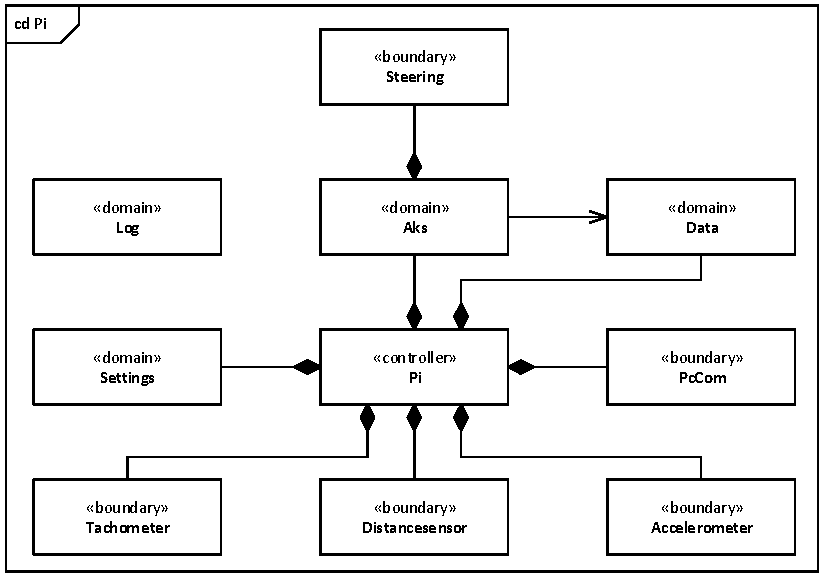
\includegraphics[width=\textwidth* 9/10]{../fig/diagrammer/bil/cd_pi.pdf}
\caption{Klassediagram over Pi}
\label{fig:cd_pi}
\end{figure}

Der gøres opmærksom på at samtlige klaser i klassediagrammet på figur \ref{fig:cd_pi} har en association til Log-klassen. Det er undladt at tegne alle disse pile, da dette vil uoverskueliggøre diagrammet.


\subsection{Pi}

Bilens styreenhed er valgt til at være en Raspberry Pi, da denne er et oplagt valg da imlementeringen både skal indeholde videostreaming og socketbaseret netværkskommunikation. Der er altså tale om en højniveau controller. Pi'en er ligeledes forsynet med et kamara\cite{lib:cam} og en Wi-Fi dongle\cite{lib:wifi}. Funktionaliteten udvikles i et program der er bestående er flere klasser, der kan ses på figur \ref{fig:cd_pi}, som herefter vil beskrives meget kort. Foruden det program som er udviklet af projektgruppen selv, anvendes et tredjepartsprogram, kaldet Motion\cite{lib:motion-on-raspberry} til at streame videoen. For flere detaljer end nedenstående henvises til \ref{P-ch:softwaredesign} \nameref{P-ch:softwaredesign} pi side \pageref{P-ch:softwaredesign} og \ref{P-ch:sw_impl} \nameref{P-ch:sw_impl} på side \pageref{P-ch:sw_impl}.

\begin{figure}[h]
\centering
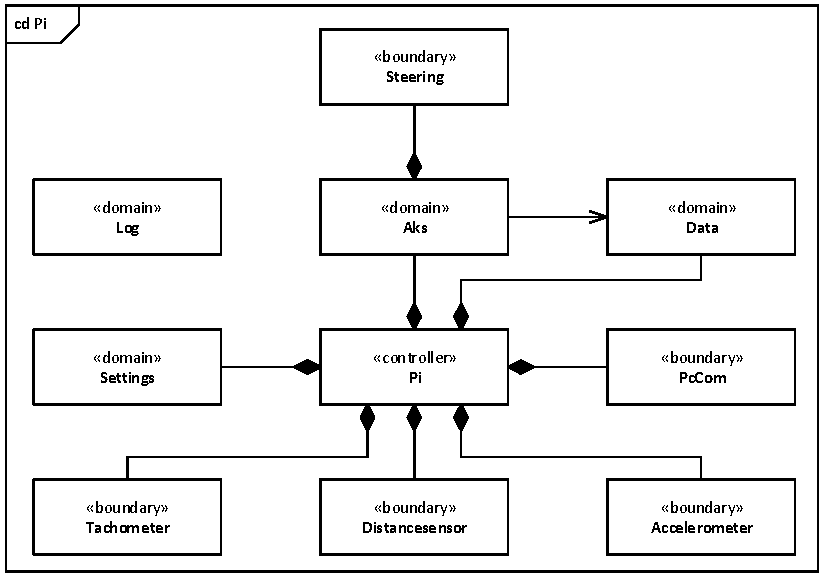
\includegraphics[width=\textwidth* 9/10]{../fig/diagrammer/bil/cd_pi.pdf}
\caption{Klassediagram over Pi}
\label{fig:cd_pi}
\end{figure}

Der gøres opmærksom på at samtlige klaser i klassediagrammet på figur \ref{fig:cd_pi} har en association til Log-klassen. Det er undladt at tegne alle disse pile, da dette vil uoverskueliggøre diagrammet.


\input{Projektbeskrivelse/SWDesign_o_impl/pi/pi/pi.tex}
\input{Projektbeskrivelse/SWDesign_o_impl/pi/aks/aks}
\input{Projektbeskrivelse/SWDesign_o_impl/pi/pccom/pccom}
\input{Projektbeskrivelse/SWDesign_o_impl/pi/settings/settings}
\input{Projektbeskrivelse/SWDesign_o_impl/pi/log/log}
\input{Projektbeskrivelse/SWDesign_o_impl/pi/data/data}
\input{Projektbeskrivelse/SWDesign_o_impl/pi/steering/steering}
\input{Projektbeskrivelse/SWDesign_o_impl/pi/psoc/psoc}

% ++++++++++++ Domain Pi AKS klassen ++++++++++++++
\subsubsection{Domain-klasse: Aks}\label{sec:aks_design}

\begin{figure}[h]
\centering
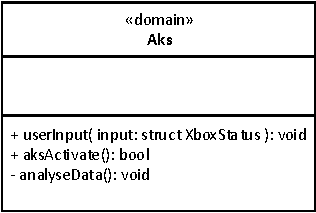
\includegraphics[scale=1]{../fig/diagrammer/bil/cd_aks.pdf}
\caption{Klassebeskrivelse for domain-klassen Aks}
\label{fig:cd_aks}
\end{figure}

\textbf{Attributter}

\begin{table}[h]
\begin{tabularx}{\textwidth}{| Z | Z | L{9cm} |} \hline
Navn & Type & Beskrivelse \\\hline
\texttt{MySteering} & \texttt{Steering} & Styretøjsklassen, bruges når Aks skal påvirke bilens hastighed eller retning.\\\hline
\texttt{MyData} & \texttt{Data*} & Pointer til bilens datastruktur.\\\hline
\texttt{MySettings} & \texttt{Settings*} & Pointer til Settingsklassen. \\\hline
\texttt{MyLog} & \texttt{Log*} & Pointer til loggen. \\\hline
\texttt{state} & \texttt{aksStates} & Husker hvilket stadie bilen er i, kan skifte mellem at stå stille, køre fremad/bagud eller trille. \\\hline
\texttt{proxSensors} & \texttt{int*} & Et array med nuværende værdier fra afstandssensorer \\\hline
\texttt{old\_proxSensors} & \texttt{int*} & Et array der holder de foregående værdier fra afstandssensorer \\\hline
\texttt{latestUserInput} & \texttt{UserInput} & Gemmer de seneste input fra brugeren. \\ \hline
\end{tabularx}
\caption{Attributter for klassen Aks}
\label{table:attr_aks}
\end{table}

\textbf{Metoder}


%----------------- aksActivate -------------------
\begin{table}[h]
\begin{tabularx}{\textwidth}{| L{2.5 cm} | Z |} \hline
Prototype & \texttt{void aksActivate(void)} \\\hline
Parametre & \texttt{void}  \\\hline
Returværdi &  \texttt{bool} \newline Returnerer \texttt{TRUE} hvis det gik godt og \texttt{FALSE} hvis der skete fejl undervejs. \\\hline
Beskrivelse & Metoden kaldes når det automatiske anti-kollisionssystem skal aktiveres. Forhindrer samtidigt input fra brugeren kortvarigt. \\\hline
\end{tabularx}
\caption{Metodebeskrivelse for \texttt{aksActivate}}
\label{table:met_aks_aksActivate}
\end{table}

%----------------- analyseData -------------------
\begin{table}[h]
\begin{tabularx}{\textwidth}{| L{2.5 cm} | Z |} \hline
Prototype & \texttt{void analyseData(void)} \\\hline
Parametre & \texttt{void}  \\\hline
Returværdi &  \texttt{void}  \\\hline
Beskrivelse & Metoden analyserer indhentet data fra Data klassen og vurderer hvilken type af undvigelse der bedst passer. Aktiverer herefter Steering-klassen for at bilen skal undvige forhindringen. \\\hline
\end{tabularx}
\caption{Metodebeskrivelse for \texttt{analyseData}}
\label{table:met_aks_analyseData}
\end{table}
\subsubsection{Boundary-klasse: PcCom} \label{sec:pccom}
PcCom klassens formål er at give mulighed for PC softwaren at skabe kontakt mellem Bil og PC. Den blev som udgangspunkt designet med en UDP protokol, men efter implementering af PC software blev dette skiftet til en TCP protokol, da softwaren var blevet implementeret således. PcCom klassen er designet og implementeret som to tråde der her især åbner en server med TCP sockets til at styre to forskellige former for datastreams mellem Bil og PC. Trådene er implementeret ved brug af biblioteket \texttt{thread}, som giver anledning til konstruktion af et object af typen \texttt{std::thread}. Disse objekter er tråde der hver især er en sekvens af instruktioner, der kan udføres sammen med andre sådanne sekvenser i multithreading miljøer. Der er under design og implementering ligeledes draget meget nytte af ''Sockets Tutorial'' \cite{lib:socket_tutorial}, en instruktion i at implemntere TCP scokets på en linux maskine.
\subsubsection{Domain-klasse: Settings} %TODO lav label

%TODO skal skrives
\subsubsection{Domain-klasse: Log}

Loggen har til formål at kunne lokalisere og identificere fejl i systemet. Loggen skal oprettes mere eller mindre globalt og der skal efterfølgende medgives en pointer til samtlige klasser på Pi. Alle disse klasser skal således anvende loggen som debugging redskab. Der skal som udgangspunkt kun skrives i loggen hvis en fejl opstår, da loggen ellers bliver uoverskuelig. Når der skrives til loggen, anvender den pågældende tråd cpu-tid, hvilket ligeledes er en grund til at være opmærksom på hvornår det er smart at skrive til loggen. \\
For at forhindre at log-entries fra forskellige tråde sammenflettes, skal der i implementeringen anvendes \texttt{std::mutex} som lås når der skrives i loggen.

\begin{figure}[h]
\centering
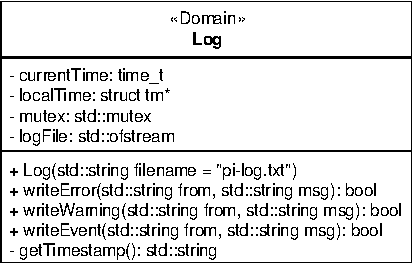
\includegraphics[]{../fig/diagrammer/bil/cd_log.pdf}
\caption{Klassebeskrivelse for domain-klassen Log}
\label{fig:cd_log}
\end{figure}

\textbf{Attributter}

\begin{table}[h]
\begin{tabularx}{\textwidth}{| Z | Z | L{10cm} |} \hline
Navn & Type & Beskrivelse \\\hline

\texttt{currentTime} & \texttt{time\_t} &Denne attribut bruges til at gemme det nuværende tidspunkt, når \texttt{getTimestamp} kaldes. \\\hline

\texttt{localTime} & \texttt{struct tm*} & Anvendes til at holde tiden i et læseligt format. \\\hline

\texttt{mutex} & \texttt{std::mutex} & Anvendes som lås i \texttt{std::lock\_guard} der forhindrer flere tråde i at skrive i loggen på samme tid. \\\hline

\texttt{logFile} & \texttt{std::ofstream} & File descriptor til logfilen. \\\hline

\end{tabularx}
\caption{Attributter for klassen Log}
\label{table:attr_log}
\end{table}


\textbf{Constructor}
%------------------------------------- Log -------------------------------------
\begin{table}[h]
\begin{tabularx}{\textwidth}{| L{2.5 cm} | Z |} \hline
Prototype & \texttt{Log(std::string filename = ''pi-log.txt'')} \\\hline
Parametre & \texttt{filename} \newline Det ønskede filnavn til logfilen der oprettes. Hvis denne parameter udelades ved initialiseringen bliver objektet oprettet med filnavnet ''pi-log.txt''.  \\\hline
Beskrivelse & Constructoren opretter et objekt af Log klassen med det angivne filnavn. \\\hline
\end{tabularx}
\caption{Beskrivelse af constructor for \texttt{Log}}
\label{table:con_log}
\end{table}

\clearpage

\textbf{Metoder}
%------------------------------------- writeError -------------------------------------
\begin{table}[h]
\begin{tabularx}{\textwidth}{| L{2.5 cm} | Z |} \hline
Prototype & \texttt{bool writeError(std::string from, std::string msg)} \\\hline
Parametre & \texttt{from} \newline Denne streng skal udfyldes med den indbyggede identifier ''\texttt{\_\_PRETTY\_FUNCTION\_\_}'' (GNU standard) der returnerer placeringen af det pågældende kald. Herved kan det i loggen ses præcis i hvilken klasse og metode log-beskeden kommer fra. \newline \newline \texttt{msg} \newline Den besked der skal stå i loggen. \\\hline
Returværdi &  \texttt{bool} \newline Returnerer \texttt{true} hvis skrivningen er gået godt og \texttt{false} hvis skrivningen gik galt. \\\hline
Beskrivelse & Metoden skriver en besked i loggen. Anvendes når der er sket en alvorlig fejl. \\\hline
\end{tabularx}
\caption{Metodebeskrivelse for \texttt{writeError}}
\label{table:met_writeError}
\end{table}

%------------------------------------- writeWarning -------------------------------------
\begin{table}[h]
\begin{tabularx}{\textwidth}{| L{2.5 cm} | Z |} \hline
Prototype & \texttt{bool writeWarning(std::string from, std::string msg)} \\\hline
Parametre & \texttt{from} \newline Denne streng skal udfyldes med den indbyggede identifier ''\texttt{\_\_PRETTY\_FUNCTION\_\_}'' (GNU standard) der returnerer placeringen af det pågældende kald. Herved kan det i loggen ses præcis i hvilken klasse og metode log-beskeden kommer fra. \newline \newline \texttt{msg} \newline Den besked der skal stå i loggen. \\\hline
Returværdi &  \texttt{bool} \newline Returnerer \texttt{true} hvis skrivningen er gået godt og \texttt{false} hvis skrivningen gik galt. \\\hline
Beskrivelse & Metoden skriver en besked i loggen. Anvendes når der er sket en mindre alvorlig fejl. \\\hline
\end{tabularx}
\caption{Metodebeskrivelse for \texttt{writeWarning}}
\label{table:met_writeWarning}
\end{table}

\clearpage

%------------------------------------- writeEvent -------------------------------------
\begin{table}[h]
\begin{tabularx}{\textwidth}{| L{2.5 cm} | Z |} \hline
Prototype & \texttt{bool writeEvent(std::string from, std::string msg)} \\\hline
Parametre & \texttt{from} \newline Denne streng skal udfyldes med den indbyggede identifier ''\texttt{\_\_PRETTY\_FUNCTION\_\_}'' (GNU standard) der returnerer placeringen af det pågældende kald. Herved kan det i loggen ses præcis i hvilken klasse og metode log-beskeden kommer fra. \newline \newline \texttt{msg} \newline Den besked der skal stå i loggen. \\\hline
Returværdi &  \texttt{bool} \newline Returnerer \texttt{true} hvis skrivningen er gået godt og \texttt{false} hvis skrivningen gik galt. \\\hline
Beskrivelse & Metoden skriver en besked i loggen. Anvendes når der er hændelse, der ikke er en fejl, som skal skrives i loggen. \\\hline
\end{tabularx}
\caption{Metodebeskrivelse for \texttt{writeEvent}}
\label{table:met_writeEvent}
\end{table}

%------------------------------------- getTimestamp -------------------------------------
\begin{table}[h]
\begin{tabularx}{\textwidth}{| L{2.5 cm} | Z |} \hline
Prototype & \texttt{std::string getTimestamp()} \\\hline
Parametre & ~ \newline \\\hline
Returværdi &  \texttt{std::string} \newline Returnerer en streng med systemets indstillede tid og dato. Formatet er \texttt{ÅÅÅÅ-MM-DD TT:MM:SS}.\\\hline
Beskrivelse & Metoden henter den nuværende tid i systemet og omdanner denne til en streng i en format der nemt kan anvendes i log-beskeder. \\\hline
\end{tabularx}
\caption{Metodebeskrivelse for \texttt{getTimestamp}}
\label{table:met_getTimestamp}
\end{table}
\subsubsection{Domain-klasse: Data} \label{sec:data_klasse}

Data-klassen indeholder alt den nyeste data, som enten skal sendes til brugerinterfacet eller som kommer fra brugerens input på Xbox-360 controlleren. Klassen har ikke anden reel funktionalitet end at beskytte data'en mod at blive korrupt hvis der er flere tråde der skriver eller læser fra den på en gang. Dette gøres ved hjælp af \texttt{std::mutex}es. Undervejs i implementeringsfasen er dette klasse testet grundigt ved brug af et stort antal tråde som alle forsøger at skrive til- o læse fra datastrukturen på samme tid.
\subsection{Steeringklassen} \label{sec:steering_impl}

Steering klassen er den klasse der kontrollere PWM signalet til motorens fremdrift og til styretøj servoen. 
Den modtager nye input fra systemet om ændringer af fremdrift, retning på styretøj og brems. Derudover henter den, hver gang klassen skal opdaterer PWM signalet til motoren, den aktuelle hastighed på bilen fra Dataklassen. 
Klassen har kun en public metode den kan kaldes. I listing \ref{lst:steering_header} ses implementering af klassens headerfilen.\newline

\lstinputlisting[linerange=Steering::header1-Steering::header2, label=lst:steering_header, caption=\texttt{Header} for Steeringklassen.]{../../src/bil/steering/steering.hpp}

Constructoen sørger primært for at sætte WiringPi op. Se sektion \ref{sec:wiringPi_impl}. 
Der er en HW og SW PWM del der skal initialiseres. 
Udover opsætning starter den en separat tråd der kører \texttt{PWMUpdate} i et loop indtil systemet lukkes ned. 
Samt at sætte værdier for PID regulering af motoren 

\lstinputlisting[linerange=Steering::Steering1-Steering::Steering2, label=lst:steering_con, caption=\texttt{Constructor} for Steeringklassen.]{../../src/bil/steering/steering.cpp}


Deconstructoen sørger for at lukke \texttt{Steering::PWMUpdate} tråden ned og joine med den, slukke for HW og SW PWM og digitale outputs til styring af H-broen.

\lstinputlisting[linerange=Steering::~Steering1-Steering::~Steering2, label=lst:steering_decon, caption=\texttt{Deconstructor} for Steeringklassen.]{../../src/bil/steering/steering.cpp}

Metoden \texttt{userInput} er den eneste metode der kan tilgås udefra. Den håndtere værdier fra Xbox 360 kontrolleren. Den omregner frem og tilbage værdierne i forhold den max hastighed der er sat for bilen. Max hastigheden hentes fra Settings klassen. Hvis der skal bremses går den direkte til \texttt{brake} metoden. Tilsidst kalder \texttt{turn} metoden

\lstinputlisting[linerange=Steering::userInput1-Steering::userInput2, label=lst:steering_userInput, caption=Metoden \texttt{userInput} Steeringklassen.]{../../src/bil/steering/steering.cpp} 

\texttt{brake} metoden bremser bilen ved at sætte motor PWM til 100 \% og de 2 retnings digitale outputs lave. Det får H-broen til at bremse motoren aktivt. Mens der bremses bliver PWM i \texttt{PWMUpdate} ikke opdateret.
\lstinputlisting[linerange=Steering::brake1-Steering::brake2, label=lst:steering_brake, caption=Metoden \texttt{brake} Steeringklassen.]{../../src/bil/steering/steering.cpp}

\texttt{softbrake} metoden sætte motor PWM til 0 \% og de 2 retnings digitale outputs lave. 
Derved vil bilen begynde at løbe farten af.
\lstinputlisting[linerange=Steering::softbrake1-Steering::softbrake2, label=lst:steering_softbrake, caption=Metoden \texttt{softbrake} Steeringklassen.]{../../src/bil/steering/steering.cpp}

\texttt{turn} metoden omregner styre værdierne fra Xbox kontrolleren til en duty cycle for SW PWM mellem 0,5ms og 2.5ms. 
Som vil give max udslag til begge sider. 
\lstinputlisting[linerange=Steering::turn1-Steering::turn2, label=lst:steering_turn, caption=Metoden \texttt{turn} Steeringklassen.]{../../src/bil/steering/steering.cpp}

\texttt{motorSetPWM} metoden bestemmer om bilen skal sættes til at kører frem eller tilbage ud fra den aktuelle retning og input fra Xbox kontrolleren. 
Hvis det er nødvendig at kører den modsatte vej bremses der indtil den er under en vis hastighed
. 
\lstinputlisting[linerange=Steering::motorSetPWM1-Steering::motorSetPWM2, label=lst:steering_motorSetPWM, caption=Metoden \texttt{motorSetPWM} Steeringklassen.]{../../src/bil/steering/steering.cpp}

\texttt{PWMUpdate} metoden kører i sin egen tråd. Den henter hver gang den aktuelle hastighed på bilen fra \texttt{Dataklassen} og udregner fejlen i forhold til den ønskede hastighed. Herefter udregner værdierne for PID reguleringen. Og til sidst sættes den nye PWM værdi på motoren. 
\lstinputlisting[linerange=Steering::PWMUpdate1-Steering::PWMUpdate2, label=lst:steering_PWMUpdate, caption=Metoden \texttt{PWMUpdate} Steeringklassen.]{../../src/bil/steering/steering.cpp}

\subsubsection{Test af Steering klassen}


\lstinputlisting[linerange=main::main1-main::main2, label=lst:steering_main, caption=Test af \texttt{Steering klassen} Steeringklassen.]{../../src/bil/steering/main.cpp}

\subsubsection*{WiringPi} \label{sec:wiringPi_impl}
\section{Psoc (PSoC)} \label{sub:sw_impl_psoc_psoc}
\subsection{Psoc (PSoC)}
PSoC'ens formål er at simplificere alt \IIC kommunikation, hvilket viste sig at være en nødvendighed, da implementeringen på Pi'en gav uforudsete problemer med kommunikationen med distancesensorerne.
Da der på Pi'en kører en Linux-distribution foregår \IIC kommunikationen som skrivning og læsning til og fra device-files der repræsenterer de respektive pins (SDA \& SCL), og da kommunikationen med distancesensorerne følger følgende protokollen fra Hardwaredesign afsnittet for distancesensoren.
Ydermere viste det sig at tachometeret, der vha. en schmittrigger trækkes til stel hver gang der detekteres en magnet, dette bliver detekteret som logisk lav på PSoC'en og  kalder den implementerede interrupt service rutine \texttt{ISR}. 
Det vil optage udnødvendig meget af Pi'ens processor og vil være meget tidskritisk i forhold til de andre opgaver som Pi-programmet varetager. Derfor beslutning om at ændre designretning.

Kravet til PSoC'en er, at koden der ligger herpå skal være så hurtig og effektiv som muligt, således at den kan aflæses når PI'en spørger på ny data. 
I listing \ref{lst:getDistance_FL2} ses implementeringen af denne kode.

\lstinputlisting
	[linerange=getDistance::FL-getDistance::FL1, caption=]
	{../../src/psoc/psoc_bil_1/psoc_bil.cydsn/main.c}

\lstinputlisting
	[linerange=getDistance::FL2-getDistance::FL3, label=lst:getDistance_FL2, caption=Front Left sensor aflæsningscyklus.]
	{../../src/psoc/psoc_bil_1/psoc_bil.cydsn/main.c}
	
aflæsningscyklus for de enkelte sensorer er identiske blot med ændret navn og index i \texttt{sendBuffer}

Tachometeret er simplere at aflæse, da alt dataen i forvejen er placeret på PSoC'en. I listing \ref{lst:sw_impl_psoc_getVelocity} ses interrupt service rutinen som køres hver gang der detekteres en magnet på hallswitchen.

\lstinputlisting
	[linerange=getVelocity::1-getVelocity::2, label=lst:sw_impl_psoc_getVelocity, caption=ISR til getVelocity.]
	{../../src/psoc/psoc_bil_1/psoc_bil.cydsn/main.c}

Til sidst kan implementeringen af programmets \texttt{main}-funktion ses i listing \ref{lst:sw_impl_psoc_main}

\lstinputlisting[linerange=main::1-main::2, label=lst:sw_impl_psoc_main, caption=Main program på PSoC.]{../../src/psoc/psoc_bil_1/psoc_bil.cydsn/main.c}

\clearpage

\subsection{Modultest for PSoC}

For at teste om kommunikationen imellem distancesensorene og PSoC'en fungerer korrekt, blev der foretaget en modultest, hvor følgende ønskedes opfyldt. 

\begin{enumerate}
  \item at der kan skrives korrekte kommander til alle 4 sensorer.
  \item at der kan læses korrekte 2-bytes værdier fra alle 4 sensorer.
\end{enumerate}

Der afvikles et main\_test program hvor der kontinuerligt skrives til de 4 sensorer én for én, og derefter læses den nuværende værdi retur i 2-bytes format. 

På figur \ref{fig:write_FL} til \ref{fig:write_RR} ses \texttt{write}-kommando sendt til alle 4 sensorer: 

\begin{figure}[h]
	\centering
	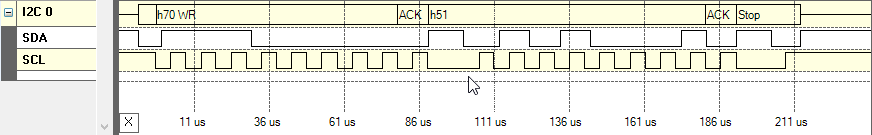
\includegraphics[scale=0.6]{../fig/billeder/psoc_distancesensor_modultest/I2C_write_0x70_FL.png}
	\caption{write til adresse 0x70 sensor FL}
	\label{fig:write_FL}
\end{figure}

\begin{figure}[h]
	\centering
	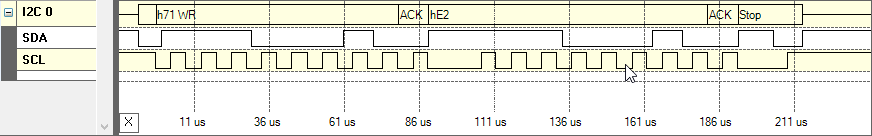
\includegraphics[scale=0.6]{../fig/billeder/psoc_distancesensor_modultest/I2C_write_0x71_FR.png}
	\caption{write til adresse 0x71 sensor FR}
	\label{fig:write_FR}
\end{figure}

\begin{figure}[h]
	\centering
	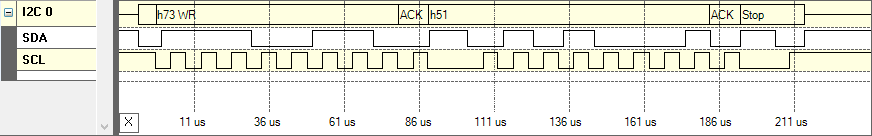
\includegraphics[scale=0.6]{../fig/billeder/psoc_distancesensor_modultest/I2C_write_0x73_RL.png}
	\caption{write til adresse 0x73 sensor RL}
	\label{fig:write_RL}
\end{figure}

\begin{figure}[h]
	\centering
	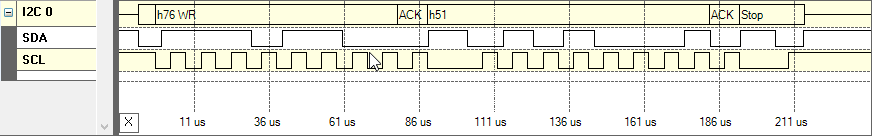
\includegraphics[scale=0.6]{../fig/billeder/psoc_distancesensor_modultest/I2C_write_0x76_RR.png}
	\caption{write til adresse 0x76 sensor RR}
	\label{fig:write_RR}
\end{figure}

\newpage

På figur \ref{fig:read_FL} til \ref{fig:read_RR} ses \texttt{read}-kommando sendt til alle 4 sensorer:

\begin{figure}[h]
	\centering
	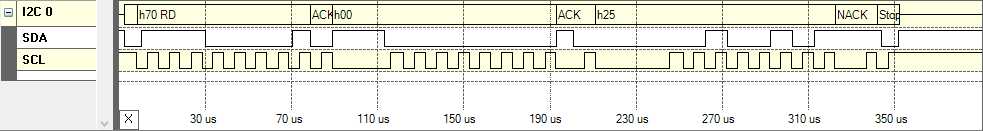
\includegraphics[scale=0.6]{../fig/billeder/psoc_distancesensor_modultest/I2C_read_0x70_FL.png}
	\caption{read til adresse 0x70 sensor FL}
	\label{fig:read_FL}
\end{figure}

\begin{figure}[h]
	\centering
	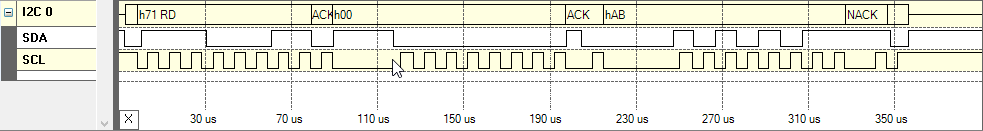
\includegraphics[scale=0.6]{../fig/billeder/psoc_distancesensor_modultest/I2C_read_0x71_FR.png}
	\caption{read til adresse 0x71 sensor FR}
	\label{fig:read_FR}
\end{figure}

\begin{figure}[h]
	\centering
	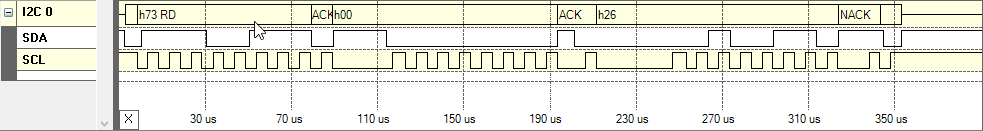
\includegraphics[scale=0.6]{../fig/billeder/psoc_distancesensor_modultest/I2C_read_0x73_RL.png}
	\caption{read til adresse 0x73 sensor RL}
	\label{fig:read_RL}
\end{figure}

\begin{figure}[h]
	\centering
	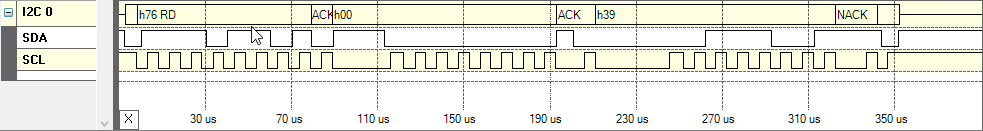
\includegraphics[scale=0.6]{../fig/billeder/psoc_distancesensor_modultest/I2C_read_0x76_RR.png}
	\caption{read til adresse 0x76 sensor RR}
	\label{fig:read_RR}
\end{figure}


% ++++++++++++ Domain Pi AKS klassen ++++++++++++++
\subsubsection{Domain-klasse: Aks}\label{sec:aks_design}

\begin{figure}[h]
\centering
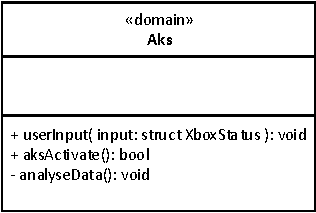
\includegraphics[scale=1]{../fig/diagrammer/bil/cd_aks.pdf}
\caption{Klassebeskrivelse for domain-klassen Aks}
\label{fig:cd_aks}
\end{figure}

\textbf{Attributter}

\begin{table}[h]
\begin{tabularx}{\textwidth}{| Z | Z | L{9cm} |} \hline
Navn & Type & Beskrivelse \\\hline
\texttt{MySteering} & \texttt{Steering} & Styretøjsklassen, bruges når Aks skal påvirke bilens hastighed eller retning.\\\hline
\texttt{MyData} & \texttt{Data*} & Pointer til bilens datastruktur.\\\hline
\texttt{MySettings} & \texttt{Settings*} & Pointer til Settingsklassen. \\\hline
\texttt{MyLog} & \texttt{Log*} & Pointer til loggen. \\\hline
\texttt{state} & \texttt{aksStates} & Husker hvilket stadie bilen er i, kan skifte mellem at stå stille, køre fremad/bagud eller trille. \\\hline
\texttt{proxSensors} & \texttt{int*} & Et array med nuværende værdier fra afstandssensorer \\\hline
\texttt{old\_proxSensors} & \texttt{int*} & Et array der holder de foregående værdier fra afstandssensorer \\\hline
\texttt{latestUserInput} & \texttt{UserInput} & Gemmer de seneste input fra brugeren. \\ \hline
\end{tabularx}
\caption{Attributter for klassen Aks}
\label{table:attr_aks}
\end{table}

\textbf{Metoder}


%----------------- aksActivate -------------------
\begin{table}[h]
\begin{tabularx}{\textwidth}{| L{2.5 cm} | Z |} \hline
Prototype & \texttt{void aksActivate(void)} \\\hline
Parametre & \texttt{void}  \\\hline
Returværdi &  \texttt{bool} \newline Returnerer \texttt{TRUE} hvis det gik godt og \texttt{FALSE} hvis der skete fejl undervejs. \\\hline
Beskrivelse & Metoden kaldes når det automatiske anti-kollisionssystem skal aktiveres. Forhindrer samtidigt input fra brugeren kortvarigt. \\\hline
\end{tabularx}
\caption{Metodebeskrivelse for \texttt{aksActivate}}
\label{table:met_aks_aksActivate}
\end{table}

%----------------- analyseData -------------------
\begin{table}[h]
\begin{tabularx}{\textwidth}{| L{2.5 cm} | Z |} \hline
Prototype & \texttt{void analyseData(void)} \\\hline
Parametre & \texttt{void}  \\\hline
Returværdi &  \texttt{void}  \\\hline
Beskrivelse & Metoden analyserer indhentet data fra Data klassen og vurderer hvilken type af undvigelse der bedst passer. Aktiverer herefter Steering-klassen for at bilen skal undvige forhindringen. \\\hline
\end{tabularx}
\caption{Metodebeskrivelse for \texttt{analyseData}}
\label{table:met_aks_analyseData}
\end{table}
\subsubsection{Boundary-klasse: PcCom} \label{sec:pccom}
PcCom klassens formål er at give mulighed for PC softwaren at skabe kontakt mellem Bil og PC. Den blev som udgangspunkt designet med en UDP protokol, men efter implementering af PC software blev dette skiftet til en TCP protokol, da softwaren var blevet implementeret således. PcCom klassen er designet og implementeret som to tråde der her især åbner en server med TCP sockets til at styre to forskellige former for datastreams mellem Bil og PC. Trådene er implementeret ved brug af biblioteket \texttt{thread}, som giver anledning til konstruktion af et object af typen \texttt{std::thread}. Disse objekter er tråde der hver især er en sekvens af instruktioner, der kan udføres sammen med andre sådanne sekvenser i multithreading miljøer. Der er under design og implementering ligeledes draget meget nytte af ''Sockets Tutorial'' \cite{lib:socket_tutorial}, en instruktion i at implemntere TCP scokets på en linux maskine.
\subsubsection{Domain-klasse: Settings} %TODO lav label

%TODO skal skrives
\subsubsection{Domain-klasse: Log}

Loggen har til formål at kunne lokalisere og identificere fejl i systemet. Loggen skal oprettes mere eller mindre globalt og der skal efterfølgende medgives en pointer til samtlige klasser på Pi. Alle disse klasser skal således anvende loggen som debugging redskab. Der skal som udgangspunkt kun skrives i loggen hvis en fejl opstår, da loggen ellers bliver uoverskuelig. Når der skrives til loggen, anvender den pågældende tråd cpu-tid, hvilket ligeledes er en grund til at være opmærksom på hvornår det er smart at skrive til loggen. \\
For at forhindre at log-entries fra forskellige tråde sammenflettes, skal der i implementeringen anvendes \texttt{std::mutex} som lås når der skrives i loggen.

\begin{figure}[h]
\centering
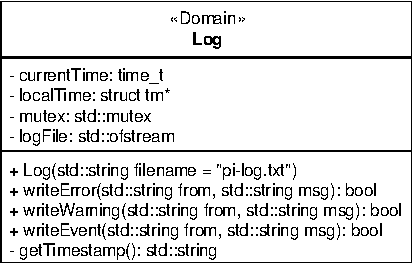
\includegraphics[]{../fig/diagrammer/bil/cd_log.pdf}
\caption{Klassebeskrivelse for domain-klassen Log}
\label{fig:cd_log}
\end{figure}

\textbf{Attributter}

\begin{table}[h]
\begin{tabularx}{\textwidth}{| Z | Z | L{10cm} |} \hline
Navn & Type & Beskrivelse \\\hline

\texttt{currentTime} & \texttt{time\_t} &Denne attribut bruges til at gemme det nuværende tidspunkt, når \texttt{getTimestamp} kaldes. \\\hline

\texttt{localTime} & \texttt{struct tm*} & Anvendes til at holde tiden i et læseligt format. \\\hline

\texttt{mutex} & \texttt{std::mutex} & Anvendes som lås i \texttt{std::lock\_guard} der forhindrer flere tråde i at skrive i loggen på samme tid. \\\hline

\texttt{logFile} & \texttt{std::ofstream} & File descriptor til logfilen. \\\hline

\end{tabularx}
\caption{Attributter for klassen Log}
\label{table:attr_log}
\end{table}


\textbf{Constructor}
%------------------------------------- Log -------------------------------------
\begin{table}[h]
\begin{tabularx}{\textwidth}{| L{2.5 cm} | Z |} \hline
Prototype & \texttt{Log(std::string filename = ''pi-log.txt'')} \\\hline
Parametre & \texttt{filename} \newline Det ønskede filnavn til logfilen der oprettes. Hvis denne parameter udelades ved initialiseringen bliver objektet oprettet med filnavnet ''pi-log.txt''.  \\\hline
Beskrivelse & Constructoren opretter et objekt af Log klassen med det angivne filnavn. \\\hline
\end{tabularx}
\caption{Beskrivelse af constructor for \texttt{Log}}
\label{table:con_log}
\end{table}

\clearpage

\textbf{Metoder}
%------------------------------------- writeError -------------------------------------
\begin{table}[h]
\begin{tabularx}{\textwidth}{| L{2.5 cm} | Z |} \hline
Prototype & \texttt{bool writeError(std::string from, std::string msg)} \\\hline
Parametre & \texttt{from} \newline Denne streng skal udfyldes med den indbyggede identifier ''\texttt{\_\_PRETTY\_FUNCTION\_\_}'' (GNU standard) der returnerer placeringen af det pågældende kald. Herved kan det i loggen ses præcis i hvilken klasse og metode log-beskeden kommer fra. \newline \newline \texttt{msg} \newline Den besked der skal stå i loggen. \\\hline
Returværdi &  \texttt{bool} \newline Returnerer \texttt{true} hvis skrivningen er gået godt og \texttt{false} hvis skrivningen gik galt. \\\hline
Beskrivelse & Metoden skriver en besked i loggen. Anvendes når der er sket en alvorlig fejl. \\\hline
\end{tabularx}
\caption{Metodebeskrivelse for \texttt{writeError}}
\label{table:met_writeError}
\end{table}

%------------------------------------- writeWarning -------------------------------------
\begin{table}[h]
\begin{tabularx}{\textwidth}{| L{2.5 cm} | Z |} \hline
Prototype & \texttt{bool writeWarning(std::string from, std::string msg)} \\\hline
Parametre & \texttt{from} \newline Denne streng skal udfyldes med den indbyggede identifier ''\texttt{\_\_PRETTY\_FUNCTION\_\_}'' (GNU standard) der returnerer placeringen af det pågældende kald. Herved kan det i loggen ses præcis i hvilken klasse og metode log-beskeden kommer fra. \newline \newline \texttt{msg} \newline Den besked der skal stå i loggen. \\\hline
Returværdi &  \texttt{bool} \newline Returnerer \texttt{true} hvis skrivningen er gået godt og \texttt{false} hvis skrivningen gik galt. \\\hline
Beskrivelse & Metoden skriver en besked i loggen. Anvendes når der er sket en mindre alvorlig fejl. \\\hline
\end{tabularx}
\caption{Metodebeskrivelse for \texttt{writeWarning}}
\label{table:met_writeWarning}
\end{table}

\clearpage

%------------------------------------- writeEvent -------------------------------------
\begin{table}[h]
\begin{tabularx}{\textwidth}{| L{2.5 cm} | Z |} \hline
Prototype & \texttt{bool writeEvent(std::string from, std::string msg)} \\\hline
Parametre & \texttt{from} \newline Denne streng skal udfyldes med den indbyggede identifier ''\texttt{\_\_PRETTY\_FUNCTION\_\_}'' (GNU standard) der returnerer placeringen af det pågældende kald. Herved kan det i loggen ses præcis i hvilken klasse og metode log-beskeden kommer fra. \newline \newline \texttt{msg} \newline Den besked der skal stå i loggen. \\\hline
Returværdi &  \texttt{bool} \newline Returnerer \texttt{true} hvis skrivningen er gået godt og \texttt{false} hvis skrivningen gik galt. \\\hline
Beskrivelse & Metoden skriver en besked i loggen. Anvendes når der er hændelse, der ikke er en fejl, som skal skrives i loggen. \\\hline
\end{tabularx}
\caption{Metodebeskrivelse for \texttt{writeEvent}}
\label{table:met_writeEvent}
\end{table}

%------------------------------------- getTimestamp -------------------------------------
\begin{table}[h]
\begin{tabularx}{\textwidth}{| L{2.5 cm} | Z |} \hline
Prototype & \texttt{std::string getTimestamp()} \\\hline
Parametre & ~ \newline \\\hline
Returværdi &  \texttt{std::string} \newline Returnerer en streng med systemets indstillede tid og dato. Formatet er \texttt{ÅÅÅÅ-MM-DD TT:MM:SS}.\\\hline
Beskrivelse & Metoden henter den nuværende tid i systemet og omdanner denne til en streng i en format der nemt kan anvendes i log-beskeder. \\\hline
\end{tabularx}
\caption{Metodebeskrivelse for \texttt{getTimestamp}}
\label{table:met_getTimestamp}
\end{table}
\subsubsection{Domain-klasse: Data} \label{sec:data_klasse}

Data-klassen indeholder alt den nyeste data, som enten skal sendes til brugerinterfacet eller som kommer fra brugerens input på Xbox-360 controlleren. Klassen har ikke anden reel funktionalitet end at beskytte data'en mod at blive korrupt hvis der er flere tråde der skriver eller læser fra den på en gang. Dette gøres ved hjælp af \texttt{std::mutex}es. Undervejs i implementeringsfasen er dette klasse testet grundigt ved brug af et stort antal tråde som alle forsøger at skrive til- o læse fra datastrukturen på samme tid.
\subsection{Steeringklassen} \label{sec:steering_impl}

Steering klassen er den klasse der kontrollere PWM signalet til motorens fremdrift og til styretøj servoen. 
Den modtager nye input fra systemet om ændringer af fremdrift, retning på styretøj og brems. Derudover henter den, hver gang klassen skal opdaterer PWM signalet til motoren, den aktuelle hastighed på bilen fra Dataklassen. 
Klassen har kun en public metode den kan kaldes. I listing \ref{lst:steering_header} ses implementering af klassens headerfilen.\newline

\lstinputlisting[linerange=Steering::header1-Steering::header2, label=lst:steering_header, caption=\texttt{Header} for Steeringklassen.]{../../src/bil/steering/steering.hpp}

Constructoen sørger primært for at sætte WiringPi op. Se sektion \ref{sec:wiringPi_impl}. 
Der er en HW og SW PWM del der skal initialiseres. 
Udover opsætning starter den en separat tråd der kører \texttt{PWMUpdate} i et loop indtil systemet lukkes ned. 
Samt at sætte værdier for PID regulering af motoren 

\lstinputlisting[linerange=Steering::Steering1-Steering::Steering2, label=lst:steering_con, caption=\texttt{Constructor} for Steeringklassen.]{../../src/bil/steering/steering.cpp}


Deconstructoen sørger for at lukke \texttt{Steering::PWMUpdate} tråden ned og joine med den, slukke for HW og SW PWM og digitale outputs til styring af H-broen.

\lstinputlisting[linerange=Steering::~Steering1-Steering::~Steering2, label=lst:steering_decon, caption=\texttt{Deconstructor} for Steeringklassen.]{../../src/bil/steering/steering.cpp}

Metoden \texttt{userInput} er den eneste metode der kan tilgås udefra. Den håndtere værdier fra Xbox 360 kontrolleren. Den omregner frem og tilbage værdierne i forhold den max hastighed der er sat for bilen. Max hastigheden hentes fra Settings klassen. Hvis der skal bremses går den direkte til \texttt{brake} metoden. Tilsidst kalder \texttt{turn} metoden

\lstinputlisting[linerange=Steering::userInput1-Steering::userInput2, label=lst:steering_userInput, caption=Metoden \texttt{userInput} Steeringklassen.]{../../src/bil/steering/steering.cpp} 

\texttt{brake} metoden bremser bilen ved at sætte motor PWM til 100 \% og de 2 retnings digitale outputs lave. Det får H-broen til at bremse motoren aktivt. Mens der bremses bliver PWM i \texttt{PWMUpdate} ikke opdateret.
\lstinputlisting[linerange=Steering::brake1-Steering::brake2, label=lst:steering_brake, caption=Metoden \texttt{brake} Steeringklassen.]{../../src/bil/steering/steering.cpp}

\texttt{softbrake} metoden sætte motor PWM til 0 \% og de 2 retnings digitale outputs lave. 
Derved vil bilen begynde at løbe farten af.
\lstinputlisting[linerange=Steering::softbrake1-Steering::softbrake2, label=lst:steering_softbrake, caption=Metoden \texttt{softbrake} Steeringklassen.]{../../src/bil/steering/steering.cpp}

\texttt{turn} metoden omregner styre værdierne fra Xbox kontrolleren til en duty cycle for SW PWM mellem 0,5ms og 2.5ms. 
Som vil give max udslag til begge sider. 
\lstinputlisting[linerange=Steering::turn1-Steering::turn2, label=lst:steering_turn, caption=Metoden \texttt{turn} Steeringklassen.]{../../src/bil/steering/steering.cpp}

\texttt{motorSetPWM} metoden bestemmer om bilen skal sættes til at kører frem eller tilbage ud fra den aktuelle retning og input fra Xbox kontrolleren. 
Hvis det er nødvendig at kører den modsatte vej bremses der indtil den er under en vis hastighed
. 
\lstinputlisting[linerange=Steering::motorSetPWM1-Steering::motorSetPWM2, label=lst:steering_motorSetPWM, caption=Metoden \texttt{motorSetPWM} Steeringklassen.]{../../src/bil/steering/steering.cpp}

\texttt{PWMUpdate} metoden kører i sin egen tråd. Den henter hver gang den aktuelle hastighed på bilen fra \texttt{Dataklassen} og udregner fejlen i forhold til den ønskede hastighed. Herefter udregner værdierne for PID reguleringen. Og til sidst sættes den nye PWM værdi på motoren. 
\lstinputlisting[linerange=Steering::PWMUpdate1-Steering::PWMUpdate2, label=lst:steering_PWMUpdate, caption=Metoden \texttt{PWMUpdate} Steeringklassen.]{../../src/bil/steering/steering.cpp}

\subsubsection{Test af Steering klassen}


\lstinputlisting[linerange=main::main1-main::main2, label=lst:steering_main, caption=Test af \texttt{Steering klassen} Steeringklassen.]{../../src/bil/steering/main.cpp}

\subsubsection*{WiringPi} \label{sec:wiringPi_impl}
\section{Psoc (PSoC)} \label{sub:sw_impl_psoc_psoc}
\subsection{Psoc (PSoC)}
PSoC'ens formål er at simplificere alt \IIC kommunikation, hvilket viste sig at være en nødvendighed, da implementeringen på Pi'en gav uforudsete problemer med kommunikationen med distancesensorerne.
Da der på Pi'en kører en Linux-distribution foregår \IIC kommunikationen som skrivning og læsning til og fra device-files der repræsenterer de respektive pins (SDA \& SCL), og da kommunikationen med distancesensorerne følger følgende protokollen fra Hardwaredesign afsnittet for distancesensoren.
Ydermere viste det sig at tachometeret, der vha. en schmittrigger trækkes til stel hver gang der detekteres en magnet, dette bliver detekteret som logisk lav på PSoC'en og  kalder den implementerede interrupt service rutine \texttt{ISR}. 
Det vil optage udnødvendig meget af Pi'ens processor og vil være meget tidskritisk i forhold til de andre opgaver som Pi-programmet varetager. Derfor beslutning om at ændre designretning.

Kravet til PSoC'en er, at koden der ligger herpå skal være så hurtig og effektiv som muligt, således at den kan aflæses når PI'en spørger på ny data. 
I listing \ref{lst:getDistance_FL2} ses implementeringen af denne kode.

\lstinputlisting
	[linerange=getDistance::FL-getDistance::FL1, caption=]
	{../../src/psoc/psoc_bil_1/psoc_bil.cydsn/main.c}

\lstinputlisting
	[linerange=getDistance::FL2-getDistance::FL3, label=lst:getDistance_FL2, caption=Front Left sensor aflæsningscyklus.]
	{../../src/psoc/psoc_bil_1/psoc_bil.cydsn/main.c}
	
aflæsningscyklus for de enkelte sensorer er identiske blot med ændret navn og index i \texttt{sendBuffer}

Tachometeret er simplere at aflæse, da alt dataen i forvejen er placeret på PSoC'en. I listing \ref{lst:sw_impl_psoc_getVelocity} ses interrupt service rutinen som køres hver gang der detekteres en magnet på hallswitchen.

\lstinputlisting
	[linerange=getVelocity::1-getVelocity::2, label=lst:sw_impl_psoc_getVelocity, caption=ISR til getVelocity.]
	{../../src/psoc/psoc_bil_1/psoc_bil.cydsn/main.c}

Til sidst kan implementeringen af programmets \texttt{main}-funktion ses i listing \ref{lst:sw_impl_psoc_main}

\lstinputlisting[linerange=main::1-main::2, label=lst:sw_impl_psoc_main, caption=Main program på PSoC.]{../../src/psoc/psoc_bil_1/psoc_bil.cydsn/main.c}

\clearpage

\subsection{Modultest for PSoC}

For at teste om kommunikationen imellem distancesensorene og PSoC'en fungerer korrekt, blev der foretaget en modultest, hvor følgende ønskedes opfyldt. 

\begin{enumerate}
  \item at der kan skrives korrekte kommander til alle 4 sensorer.
  \item at der kan læses korrekte 2-bytes værdier fra alle 4 sensorer.
\end{enumerate}

Der afvikles et main\_test program hvor der kontinuerligt skrives til de 4 sensorer én for én, og derefter læses den nuværende værdi retur i 2-bytes format. 

På figur \ref{fig:write_FL} til \ref{fig:write_RR} ses \texttt{write}-kommando sendt til alle 4 sensorer: 

\begin{figure}[h]
	\centering
	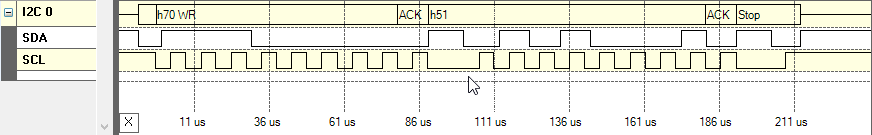
\includegraphics[scale=0.6]{../fig/billeder/psoc_distancesensor_modultest/I2C_write_0x70_FL.png}
	\caption{write til adresse 0x70 sensor FL}
	\label{fig:write_FL}
\end{figure}

\begin{figure}[h]
	\centering
	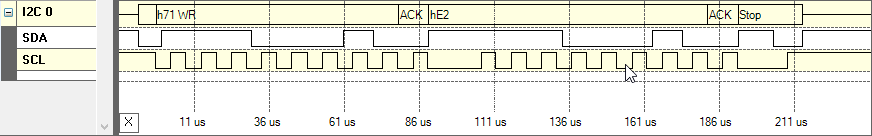
\includegraphics[scale=0.6]{../fig/billeder/psoc_distancesensor_modultest/I2C_write_0x71_FR.png}
	\caption{write til adresse 0x71 sensor FR}
	\label{fig:write_FR}
\end{figure}

\begin{figure}[h]
	\centering
	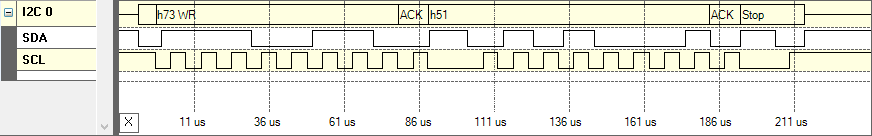
\includegraphics[scale=0.6]{../fig/billeder/psoc_distancesensor_modultest/I2C_write_0x73_RL.png}
	\caption{write til adresse 0x73 sensor RL}
	\label{fig:write_RL}
\end{figure}

\begin{figure}[h]
	\centering
	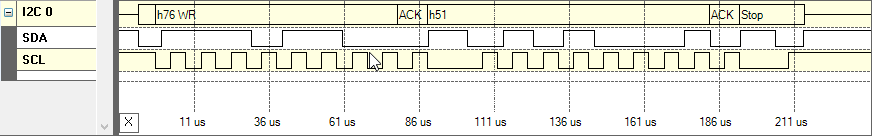
\includegraphics[scale=0.6]{../fig/billeder/psoc_distancesensor_modultest/I2C_write_0x76_RR.png}
	\caption{write til adresse 0x76 sensor RR}
	\label{fig:write_RR}
\end{figure}

\newpage

På figur \ref{fig:read_FL} til \ref{fig:read_RR} ses \texttt{read}-kommando sendt til alle 4 sensorer:

\begin{figure}[h]
	\centering
	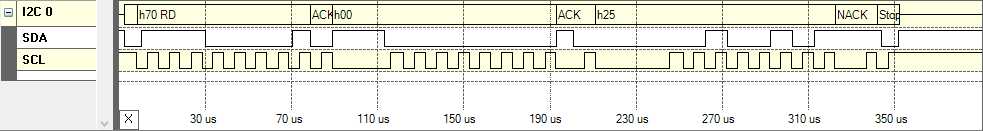
\includegraphics[scale=0.6]{../fig/billeder/psoc_distancesensor_modultest/I2C_read_0x70_FL.png}
	\caption{read til adresse 0x70 sensor FL}
	\label{fig:read_FL}
\end{figure}

\begin{figure}[h]
	\centering
	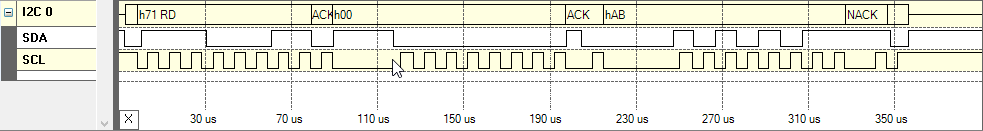
\includegraphics[scale=0.6]{../fig/billeder/psoc_distancesensor_modultest/I2C_read_0x71_FR.png}
	\caption{read til adresse 0x71 sensor FR}
	\label{fig:read_FR}
\end{figure}

\begin{figure}[h]
	\centering
	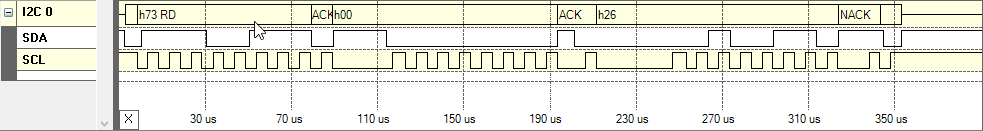
\includegraphics[scale=0.6]{../fig/billeder/psoc_distancesensor_modultest/I2C_read_0x73_RL.png}
	\caption{read til adresse 0x73 sensor RL}
	\label{fig:read_RL}
\end{figure}

\begin{figure}[h]
	\centering
	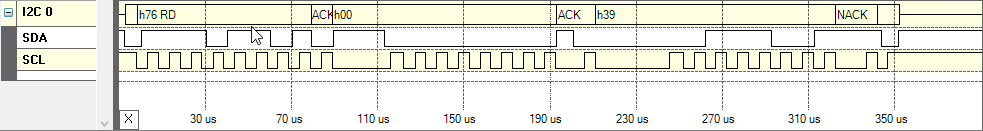
\includegraphics[scale=0.6]{../fig/billeder/psoc_distancesensor_modultest/I2C_read_0x76_RR.png}
	\caption{read til adresse 0x76 sensor RR}
	\label{fig:read_RR}
\end{figure}


% ++++++++++++ Domain Pi AKS klassen ++++++++++++++
\subsubsection{Domain-klasse: Aks}\label{sec:aks_design}

\begin{figure}[h]
\centering
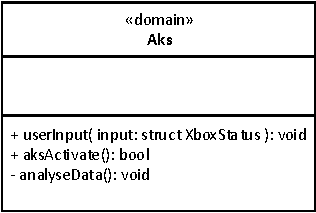
\includegraphics[scale=1]{../fig/diagrammer/bil/cd_aks.pdf}
\caption{Klassebeskrivelse for domain-klassen Aks}
\label{fig:cd_aks}
\end{figure}

\textbf{Attributter}

\begin{table}[h]
\begin{tabularx}{\textwidth}{| Z | Z | L{9cm} |} \hline
Navn & Type & Beskrivelse \\\hline
\texttt{MySteering} & \texttt{Steering} & Styretøjsklassen, bruges når Aks skal påvirke bilens hastighed eller retning.\\\hline
\texttt{MyData} & \texttt{Data*} & Pointer til bilens datastruktur.\\\hline
\texttt{MySettings} & \texttt{Settings*} & Pointer til Settingsklassen. \\\hline
\texttt{MyLog} & \texttt{Log*} & Pointer til loggen. \\\hline
\texttt{state} & \texttt{aksStates} & Husker hvilket stadie bilen er i, kan skifte mellem at stå stille, køre fremad/bagud eller trille. \\\hline
\texttt{proxSensors} & \texttt{int*} & Et array med nuværende værdier fra afstandssensorer \\\hline
\texttt{old\_proxSensors} & \texttt{int*} & Et array der holder de foregående værdier fra afstandssensorer \\\hline
\texttt{latestUserInput} & \texttt{UserInput} & Gemmer de seneste input fra brugeren. \\ \hline
\end{tabularx}
\caption{Attributter for klassen Aks}
\label{table:attr_aks}
\end{table}

\textbf{Metoder}


%----------------- aksActivate -------------------
\begin{table}[h]
\begin{tabularx}{\textwidth}{| L{2.5 cm} | Z |} \hline
Prototype & \texttt{void aksActivate(void)} \\\hline
Parametre & \texttt{void}  \\\hline
Returværdi &  \texttt{bool} \newline Returnerer \texttt{TRUE} hvis det gik godt og \texttt{FALSE} hvis der skete fejl undervejs. \\\hline
Beskrivelse & Metoden kaldes når det automatiske anti-kollisionssystem skal aktiveres. Forhindrer samtidigt input fra brugeren kortvarigt. \\\hline
\end{tabularx}
\caption{Metodebeskrivelse for \texttt{aksActivate}}
\label{table:met_aks_aksActivate}
\end{table}

%----------------- analyseData -------------------
\begin{table}[h]
\begin{tabularx}{\textwidth}{| L{2.5 cm} | Z |} \hline
Prototype & \texttt{void analyseData(void)} \\\hline
Parametre & \texttt{void}  \\\hline
Returværdi &  \texttt{void}  \\\hline
Beskrivelse & Metoden analyserer indhentet data fra Data klassen og vurderer hvilken type af undvigelse der bedst passer. Aktiverer herefter Steering-klassen for at bilen skal undvige forhindringen. \\\hline
\end{tabularx}
\caption{Metodebeskrivelse for \texttt{analyseData}}
\label{table:met_aks_analyseData}
\end{table}
\subsubsection{Boundary-klasse: PcCom} \label{sec:pccom}
PcCom klassens formål er at give mulighed for PC softwaren at skabe kontakt mellem Bil og PC. Den blev som udgangspunkt designet med en UDP protokol, men efter implementering af PC software blev dette skiftet til en TCP protokol, da softwaren var blevet implementeret således. PcCom klassen er designet og implementeret som to tråde der her især åbner en server med TCP sockets til at styre to forskellige former for datastreams mellem Bil og PC. Trådene er implementeret ved brug af biblioteket \texttt{thread}, som giver anledning til konstruktion af et object af typen \texttt{std::thread}. Disse objekter er tråde der hver især er en sekvens af instruktioner, der kan udføres sammen med andre sådanne sekvenser i multithreading miljøer. Der er under design og implementering ligeledes draget meget nytte af ''Sockets Tutorial'' \cite{lib:socket_tutorial}, en instruktion i at implemntere TCP scokets på en linux maskine.
\subsubsection{Domain-klasse: Settings} %TODO lav label

%TODO skal skrives
\subsubsection{Domain-klasse: Log}

Loggen har til formål at kunne lokalisere og identificere fejl i systemet. Loggen skal oprettes mere eller mindre globalt og der skal efterfølgende medgives en pointer til samtlige klasser på Pi. Alle disse klasser skal således anvende loggen som debugging redskab. Der skal som udgangspunkt kun skrives i loggen hvis en fejl opstår, da loggen ellers bliver uoverskuelig. Når der skrives til loggen, anvender den pågældende tråd cpu-tid, hvilket ligeledes er en grund til at være opmærksom på hvornår det er smart at skrive til loggen. \\
For at forhindre at log-entries fra forskellige tråde sammenflettes, skal der i implementeringen anvendes \texttt{std::mutex} som lås når der skrives i loggen.

\begin{figure}[h]
\centering
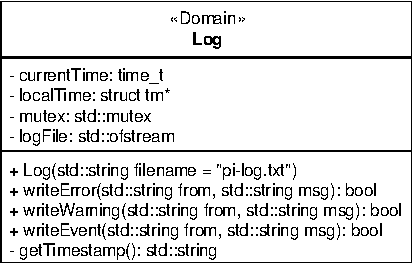
\includegraphics[]{../fig/diagrammer/bil/cd_log.pdf}
\caption{Klassebeskrivelse for domain-klassen Log}
\label{fig:cd_log}
\end{figure}

\textbf{Attributter}

\begin{table}[h]
\begin{tabularx}{\textwidth}{| Z | Z | L{10cm} |} \hline
Navn & Type & Beskrivelse \\\hline

\texttt{currentTime} & \texttt{time\_t} &Denne attribut bruges til at gemme det nuværende tidspunkt, når \texttt{getTimestamp} kaldes. \\\hline

\texttt{localTime} & \texttt{struct tm*} & Anvendes til at holde tiden i et læseligt format. \\\hline

\texttt{mutex} & \texttt{std::mutex} & Anvendes som lås i \texttt{std::lock\_guard} der forhindrer flere tråde i at skrive i loggen på samme tid. \\\hline

\texttt{logFile} & \texttt{std::ofstream} & File descriptor til logfilen. \\\hline

\end{tabularx}
\caption{Attributter for klassen Log}
\label{table:attr_log}
\end{table}


\textbf{Constructor}
%------------------------------------- Log -------------------------------------
\begin{table}[h]
\begin{tabularx}{\textwidth}{| L{2.5 cm} | Z |} \hline
Prototype & \texttt{Log(std::string filename = ''pi-log.txt'')} \\\hline
Parametre & \texttt{filename} \newline Det ønskede filnavn til logfilen der oprettes. Hvis denne parameter udelades ved initialiseringen bliver objektet oprettet med filnavnet ''pi-log.txt''.  \\\hline
Beskrivelse & Constructoren opretter et objekt af Log klassen med det angivne filnavn. \\\hline
\end{tabularx}
\caption{Beskrivelse af constructor for \texttt{Log}}
\label{table:con_log}
\end{table}

\clearpage

\textbf{Metoder}
%------------------------------------- writeError -------------------------------------
\begin{table}[h]
\begin{tabularx}{\textwidth}{| L{2.5 cm} | Z |} \hline
Prototype & \texttt{bool writeError(std::string from, std::string msg)} \\\hline
Parametre & \texttt{from} \newline Denne streng skal udfyldes med den indbyggede identifier ''\texttt{\_\_PRETTY\_FUNCTION\_\_}'' (GNU standard) der returnerer placeringen af det pågældende kald. Herved kan det i loggen ses præcis i hvilken klasse og metode log-beskeden kommer fra. \newline \newline \texttt{msg} \newline Den besked der skal stå i loggen. \\\hline
Returværdi &  \texttt{bool} \newline Returnerer \texttt{true} hvis skrivningen er gået godt og \texttt{false} hvis skrivningen gik galt. \\\hline
Beskrivelse & Metoden skriver en besked i loggen. Anvendes når der er sket en alvorlig fejl. \\\hline
\end{tabularx}
\caption{Metodebeskrivelse for \texttt{writeError}}
\label{table:met_writeError}
\end{table}

%------------------------------------- writeWarning -------------------------------------
\begin{table}[h]
\begin{tabularx}{\textwidth}{| L{2.5 cm} | Z |} \hline
Prototype & \texttt{bool writeWarning(std::string from, std::string msg)} \\\hline
Parametre & \texttt{from} \newline Denne streng skal udfyldes med den indbyggede identifier ''\texttt{\_\_PRETTY\_FUNCTION\_\_}'' (GNU standard) der returnerer placeringen af det pågældende kald. Herved kan det i loggen ses præcis i hvilken klasse og metode log-beskeden kommer fra. \newline \newline \texttt{msg} \newline Den besked der skal stå i loggen. \\\hline
Returværdi &  \texttt{bool} \newline Returnerer \texttt{true} hvis skrivningen er gået godt og \texttt{false} hvis skrivningen gik galt. \\\hline
Beskrivelse & Metoden skriver en besked i loggen. Anvendes når der er sket en mindre alvorlig fejl. \\\hline
\end{tabularx}
\caption{Metodebeskrivelse for \texttt{writeWarning}}
\label{table:met_writeWarning}
\end{table}

\clearpage

%------------------------------------- writeEvent -------------------------------------
\begin{table}[h]
\begin{tabularx}{\textwidth}{| L{2.5 cm} | Z |} \hline
Prototype & \texttt{bool writeEvent(std::string from, std::string msg)} \\\hline
Parametre & \texttt{from} \newline Denne streng skal udfyldes med den indbyggede identifier ''\texttt{\_\_PRETTY\_FUNCTION\_\_}'' (GNU standard) der returnerer placeringen af det pågældende kald. Herved kan det i loggen ses præcis i hvilken klasse og metode log-beskeden kommer fra. \newline \newline \texttt{msg} \newline Den besked der skal stå i loggen. \\\hline
Returværdi &  \texttt{bool} \newline Returnerer \texttt{true} hvis skrivningen er gået godt og \texttt{false} hvis skrivningen gik galt. \\\hline
Beskrivelse & Metoden skriver en besked i loggen. Anvendes når der er hændelse, der ikke er en fejl, som skal skrives i loggen. \\\hline
\end{tabularx}
\caption{Metodebeskrivelse for \texttt{writeEvent}}
\label{table:met_writeEvent}
\end{table}

%------------------------------------- getTimestamp -------------------------------------
\begin{table}[h]
\begin{tabularx}{\textwidth}{| L{2.5 cm} | Z |} \hline
Prototype & \texttt{std::string getTimestamp()} \\\hline
Parametre & ~ \newline \\\hline
Returværdi &  \texttt{std::string} \newline Returnerer en streng med systemets indstillede tid og dato. Formatet er \texttt{ÅÅÅÅ-MM-DD TT:MM:SS}.\\\hline
Beskrivelse & Metoden henter den nuværende tid i systemet og omdanner denne til en streng i en format der nemt kan anvendes i log-beskeder. \\\hline
\end{tabularx}
\caption{Metodebeskrivelse for \texttt{getTimestamp}}
\label{table:met_getTimestamp}
\end{table}
\subsubsection{Domain-klasse: Data} \label{sec:data_klasse}

Data-klassen indeholder alt den nyeste data, som enten skal sendes til brugerinterfacet eller som kommer fra brugerens input på Xbox-360 controlleren. Klassen har ikke anden reel funktionalitet end at beskytte data'en mod at blive korrupt hvis der er flere tråde der skriver eller læser fra den på en gang. Dette gøres ved hjælp af \texttt{std::mutex}es. Undervejs i implementeringsfasen er dette klasse testet grundigt ved brug af et stort antal tråde som alle forsøger at skrive til- o læse fra datastrukturen på samme tid.
\subsubsection{Boundary-klasse: Accelerometer} %TODO lav label

%TODO skal skrives
\subsection{Steeringklassen} \label{sec:steering_impl}

Steering klassen er den klasse der kontrollere PWM signalet til motorens fremdrift og til styretøj servoen. 
Den modtager nye input fra systemet om ændringer af fremdrift, retning på styretøj og brems. Derudover henter den, hver gang klassen skal opdaterer PWM signalet til motoren, den aktuelle hastighed på bilen fra Dataklassen. 
Klassen har kun en public metode den kan kaldes. I listing \ref{lst:steering_header} ses implementering af klassens headerfilen.\newline

\lstinputlisting[linerange=Steering::header1-Steering::header2, label=lst:steering_header, caption=\texttt{Header} for Steeringklassen.]{../../src/bil/steering/steering.hpp}

Constructoen sørger primært for at sætte WiringPi op. Se sektion \ref{sec:wiringPi_impl}. 
Der er en HW og SW PWM del der skal initialiseres. 
Udover opsætning starter den en separat tråd der kører \texttt{PWMUpdate} i et loop indtil systemet lukkes ned. 
Samt at sætte værdier for PID regulering af motoren 

\lstinputlisting[linerange=Steering::Steering1-Steering::Steering2, label=lst:steering_con, caption=\texttt{Constructor} for Steeringklassen.]{../../src/bil/steering/steering.cpp}


Deconstructoen sørger for at lukke \texttt{Steering::PWMUpdate} tråden ned og joine med den, slukke for HW og SW PWM og digitale outputs til styring af H-broen.

\lstinputlisting[linerange=Steering::~Steering1-Steering::~Steering2, label=lst:steering_decon, caption=\texttt{Deconstructor} for Steeringklassen.]{../../src/bil/steering/steering.cpp}

Metoden \texttt{userInput} er den eneste metode der kan tilgås udefra. Den håndtere værdier fra Xbox 360 kontrolleren. Den omregner frem og tilbage værdierne i forhold den max hastighed der er sat for bilen. Max hastigheden hentes fra Settings klassen. Hvis der skal bremses går den direkte til \texttt{brake} metoden. Tilsidst kalder \texttt{turn} metoden

\lstinputlisting[linerange=Steering::userInput1-Steering::userInput2, label=lst:steering_userInput, caption=Metoden \texttt{userInput} Steeringklassen.]{../../src/bil/steering/steering.cpp} 

\texttt{brake} metoden bremser bilen ved at sætte motor PWM til 100 \% og de 2 retnings digitale outputs lave. Det får H-broen til at bremse motoren aktivt. Mens der bremses bliver PWM i \texttt{PWMUpdate} ikke opdateret.
\lstinputlisting[linerange=Steering::brake1-Steering::brake2, label=lst:steering_brake, caption=Metoden \texttt{brake} Steeringklassen.]{../../src/bil/steering/steering.cpp}

\texttt{softbrake} metoden sætte motor PWM til 0 \% og de 2 retnings digitale outputs lave. 
Derved vil bilen begynde at løbe farten af.
\lstinputlisting[linerange=Steering::softbrake1-Steering::softbrake2, label=lst:steering_softbrake, caption=Metoden \texttt{softbrake} Steeringklassen.]{../../src/bil/steering/steering.cpp}

\texttt{turn} metoden omregner styre værdierne fra Xbox kontrolleren til en duty cycle for SW PWM mellem 0,5ms og 2.5ms. 
Som vil give max udslag til begge sider. 
\lstinputlisting[linerange=Steering::turn1-Steering::turn2, label=lst:steering_turn, caption=Metoden \texttt{turn} Steeringklassen.]{../../src/bil/steering/steering.cpp}

\texttt{motorSetPWM} metoden bestemmer om bilen skal sættes til at kører frem eller tilbage ud fra den aktuelle retning og input fra Xbox kontrolleren. 
Hvis det er nødvendig at kører den modsatte vej bremses der indtil den er under en vis hastighed
. 
\lstinputlisting[linerange=Steering::motorSetPWM1-Steering::motorSetPWM2, label=lst:steering_motorSetPWM, caption=Metoden \texttt{motorSetPWM} Steeringklassen.]{../../src/bil/steering/steering.cpp}

\texttt{PWMUpdate} metoden kører i sin egen tråd. Den henter hver gang den aktuelle hastighed på bilen fra \texttt{Dataklassen} og udregner fejlen i forhold til den ønskede hastighed. Herefter udregner værdierne for PID reguleringen. Og til sidst sættes den nye PWM værdi på motoren. 
\lstinputlisting[linerange=Steering::PWMUpdate1-Steering::PWMUpdate2, label=lst:steering_PWMUpdate, caption=Metoden \texttt{PWMUpdate} Steeringklassen.]{../../src/bil/steering/steering.cpp}

\subsubsection{Test af Steering klassen}


\lstinputlisting[linerange=main::main1-main::main2, label=lst:steering_main, caption=Test af \texttt{Steering klassen} Steeringklassen.]{../../src/bil/steering/main.cpp}

\subsubsection*{WiringPi} \label{sec:wiringPi_impl}
\section{Psoc (PSoC)} \label{sub:sw_impl_psoc_psoc}
\subsection{Psoc (PSoC)}
PSoC'ens formål er at simplificere alt \IIC kommunikation, hvilket viste sig at være en nødvendighed, da implementeringen på Pi'en gav uforudsete problemer med kommunikationen med distancesensorerne.
Da der på Pi'en kører en Linux-distribution foregår \IIC kommunikationen som skrivning og læsning til og fra device-files der repræsenterer de respektive pins (SDA \& SCL), og da kommunikationen med distancesensorerne følger følgende protokollen fra Hardwaredesign afsnittet for distancesensoren.
Ydermere viste det sig at tachometeret, der vha. en schmittrigger trækkes til stel hver gang der detekteres en magnet, dette bliver detekteret som logisk lav på PSoC'en og  kalder den implementerede interrupt service rutine \texttt{ISR}. 
Det vil optage udnødvendig meget af Pi'ens processor og vil være meget tidskritisk i forhold til de andre opgaver som Pi-programmet varetager. Derfor beslutning om at ændre designretning.

Kravet til PSoC'en er, at koden der ligger herpå skal være så hurtig og effektiv som muligt, således at den kan aflæses når PI'en spørger på ny data. 
I listing \ref{lst:getDistance_FL2} ses implementeringen af denne kode.

\lstinputlisting
	[linerange=getDistance::FL-getDistance::FL1, caption=]
	{../../src/psoc/psoc_bil_1/psoc_bil.cydsn/main.c}

\lstinputlisting
	[linerange=getDistance::FL2-getDistance::FL3, label=lst:getDistance_FL2, caption=Front Left sensor aflæsningscyklus.]
	{../../src/psoc/psoc_bil_1/psoc_bil.cydsn/main.c}
	
aflæsningscyklus for de enkelte sensorer er identiske blot med ændret navn og index i \texttt{sendBuffer}

Tachometeret er simplere at aflæse, da alt dataen i forvejen er placeret på PSoC'en. I listing \ref{lst:sw_impl_psoc_getVelocity} ses interrupt service rutinen som køres hver gang der detekteres en magnet på hallswitchen.

\lstinputlisting
	[linerange=getVelocity::1-getVelocity::2, label=lst:sw_impl_psoc_getVelocity, caption=ISR til getVelocity.]
	{../../src/psoc/psoc_bil_1/psoc_bil.cydsn/main.c}

Til sidst kan implementeringen af programmets \texttt{main}-funktion ses i listing \ref{lst:sw_impl_psoc_main}

\lstinputlisting[linerange=main::1-main::2, label=lst:sw_impl_psoc_main, caption=Main program på PSoC.]{../../src/psoc/psoc_bil_1/psoc_bil.cydsn/main.c}

\clearpage

\subsection{Modultest for PSoC}

For at teste om kommunikationen imellem distancesensorene og PSoC'en fungerer korrekt, blev der foretaget en modultest, hvor følgende ønskedes opfyldt. 

\begin{enumerate}
  \item at der kan skrives korrekte kommander til alle 4 sensorer.
  \item at der kan læses korrekte 2-bytes værdier fra alle 4 sensorer.
\end{enumerate}

Der afvikles et main\_test program hvor der kontinuerligt skrives til de 4 sensorer én for én, og derefter læses den nuværende værdi retur i 2-bytes format. 

På figur \ref{fig:write_FL} til \ref{fig:write_RR} ses \texttt{write}-kommando sendt til alle 4 sensorer: 

\begin{figure}[h]
	\centering
	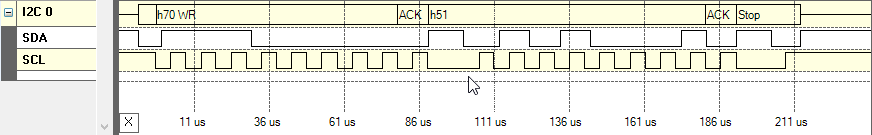
\includegraphics[scale=0.6]{../fig/billeder/psoc_distancesensor_modultest/I2C_write_0x70_FL.png}
	\caption{write til adresse 0x70 sensor FL}
	\label{fig:write_FL}
\end{figure}

\begin{figure}[h]
	\centering
	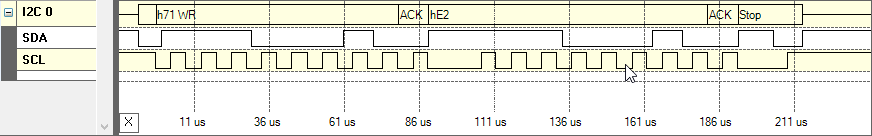
\includegraphics[scale=0.6]{../fig/billeder/psoc_distancesensor_modultest/I2C_write_0x71_FR.png}
	\caption{write til adresse 0x71 sensor FR}
	\label{fig:write_FR}
\end{figure}

\begin{figure}[h]
	\centering
	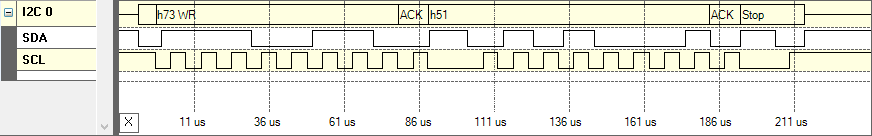
\includegraphics[scale=0.6]{../fig/billeder/psoc_distancesensor_modultest/I2C_write_0x73_RL.png}
	\caption{write til adresse 0x73 sensor RL}
	\label{fig:write_RL}
\end{figure}

\begin{figure}[h]
	\centering
	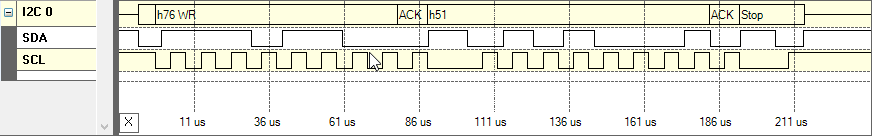
\includegraphics[scale=0.6]{../fig/billeder/psoc_distancesensor_modultest/I2C_write_0x76_RR.png}
	\caption{write til adresse 0x76 sensor RR}
	\label{fig:write_RR}
\end{figure}

\newpage

På figur \ref{fig:read_FL} til \ref{fig:read_RR} ses \texttt{read}-kommando sendt til alle 4 sensorer:

\begin{figure}[h]
	\centering
	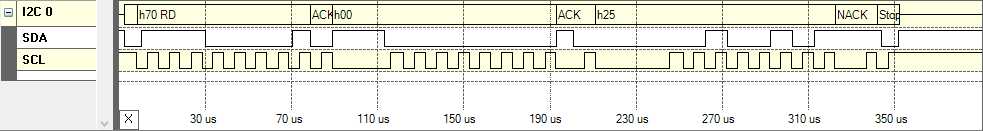
\includegraphics[scale=0.6]{../fig/billeder/psoc_distancesensor_modultest/I2C_read_0x70_FL.png}
	\caption{read til adresse 0x70 sensor FL}
	\label{fig:read_FL}
\end{figure}

\begin{figure}[h]
	\centering
	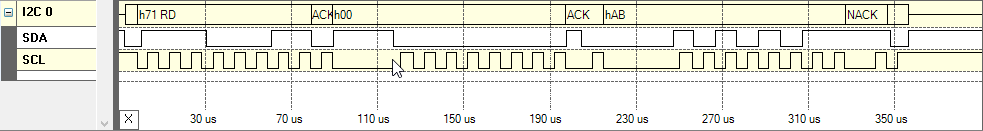
\includegraphics[scale=0.6]{../fig/billeder/psoc_distancesensor_modultest/I2C_read_0x71_FR.png}
	\caption{read til adresse 0x71 sensor FR}
	\label{fig:read_FR}
\end{figure}

\begin{figure}[h]
	\centering
	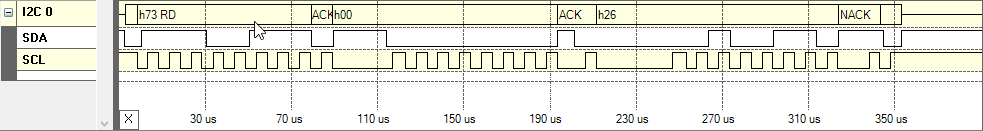
\includegraphics[scale=0.6]{../fig/billeder/psoc_distancesensor_modultest/I2C_read_0x73_RL.png}
	\caption{read til adresse 0x73 sensor RL}
	\label{fig:read_RL}
\end{figure}

\begin{figure}[h]
	\centering
	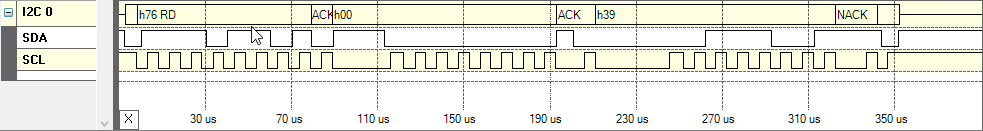
\includegraphics[scale=0.6]{../fig/billeder/psoc_distancesensor_modultest/I2C_read_0x76_RR.png}
	\caption{read til adresse 0x76 sensor RR}
	\label{fig:read_RR}
\end{figure}

